%!TEX root = ../report.tex
\documentclass[../report.tex]{subfiles}

\begin{document}
\section{Manual Motion Observation }
\label{sec:exp01}
The goal of this experiment is to design a differntial drive robot using LEGO EV3 and then measure its pose variation for three different constant velocity motions: an arc to the left, straight line ahead, and an arc to the right.
\subsection{Design of Experiment}

A differential drive robot is a mobile robot that moves using two independently driven wheels mounted on either side of its chassis. By varying the relative speed and direction of these wheels, the robot can move forward, backward, or rotate in place, making it highly maneuverable. This design is simple, cost-effective, and widely used in research and industry for tasks such as navigation, mapping, and control experiments.


\begin{figure}[ht]
        \centering
        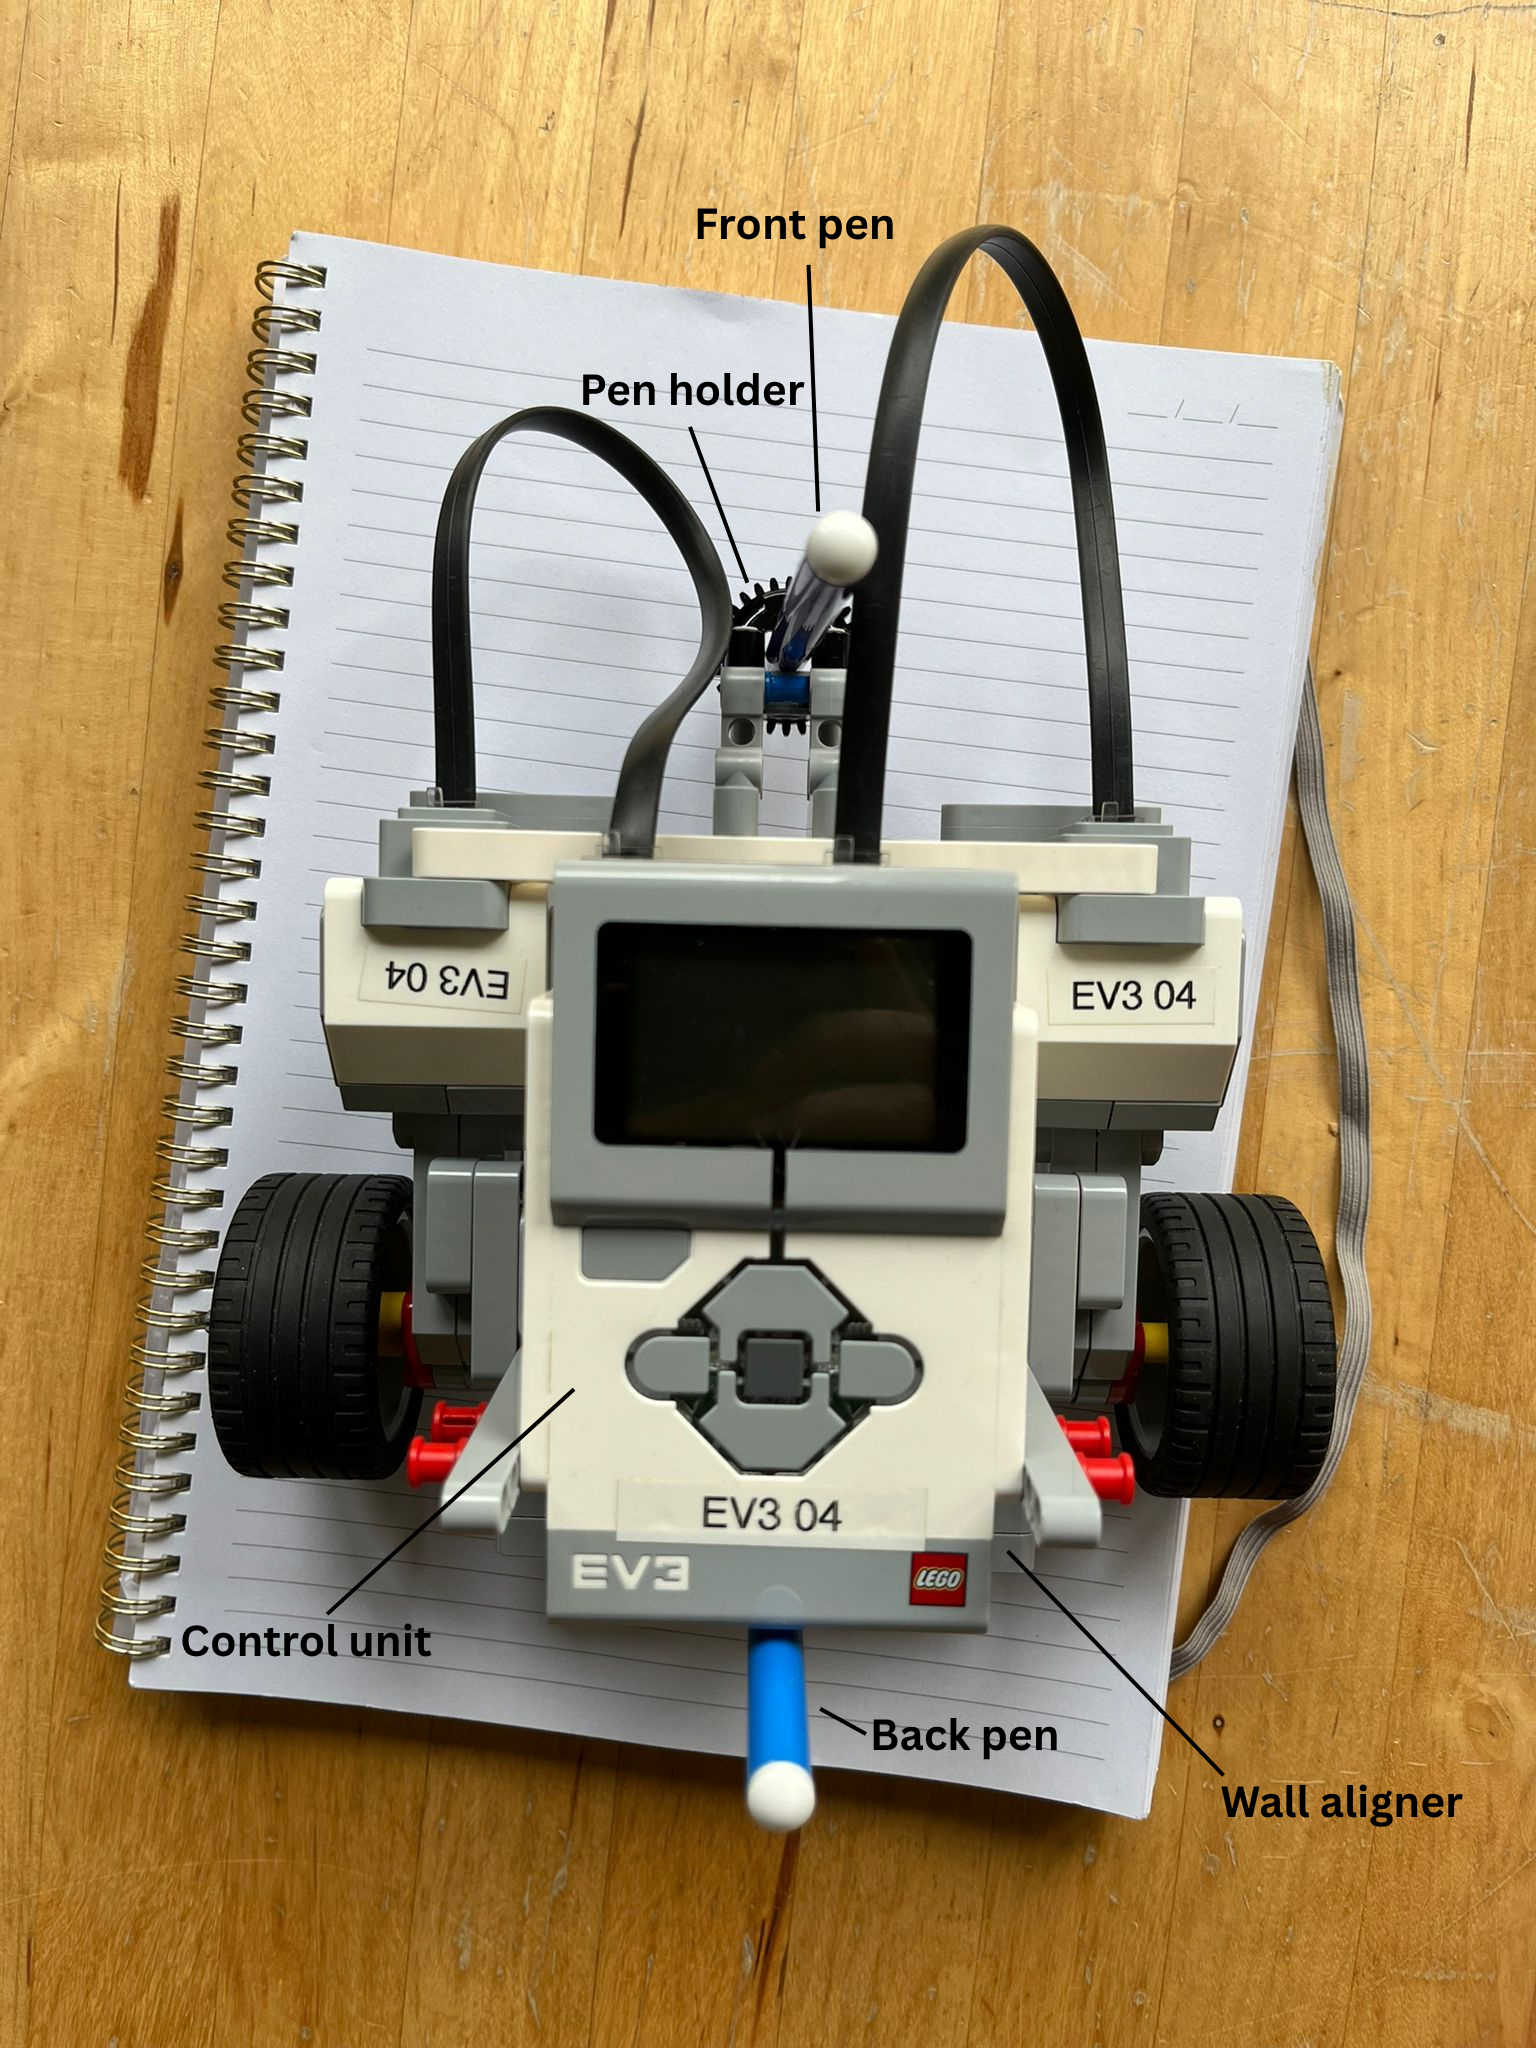
\includegraphics[width=0.8\linewidth]{figures/robot_angles/top.png}
        \caption{Top view of the robot}
        \label{fig:top_view}
    \end{figure}
    
    \begin{figure}[ht]
        \centering
        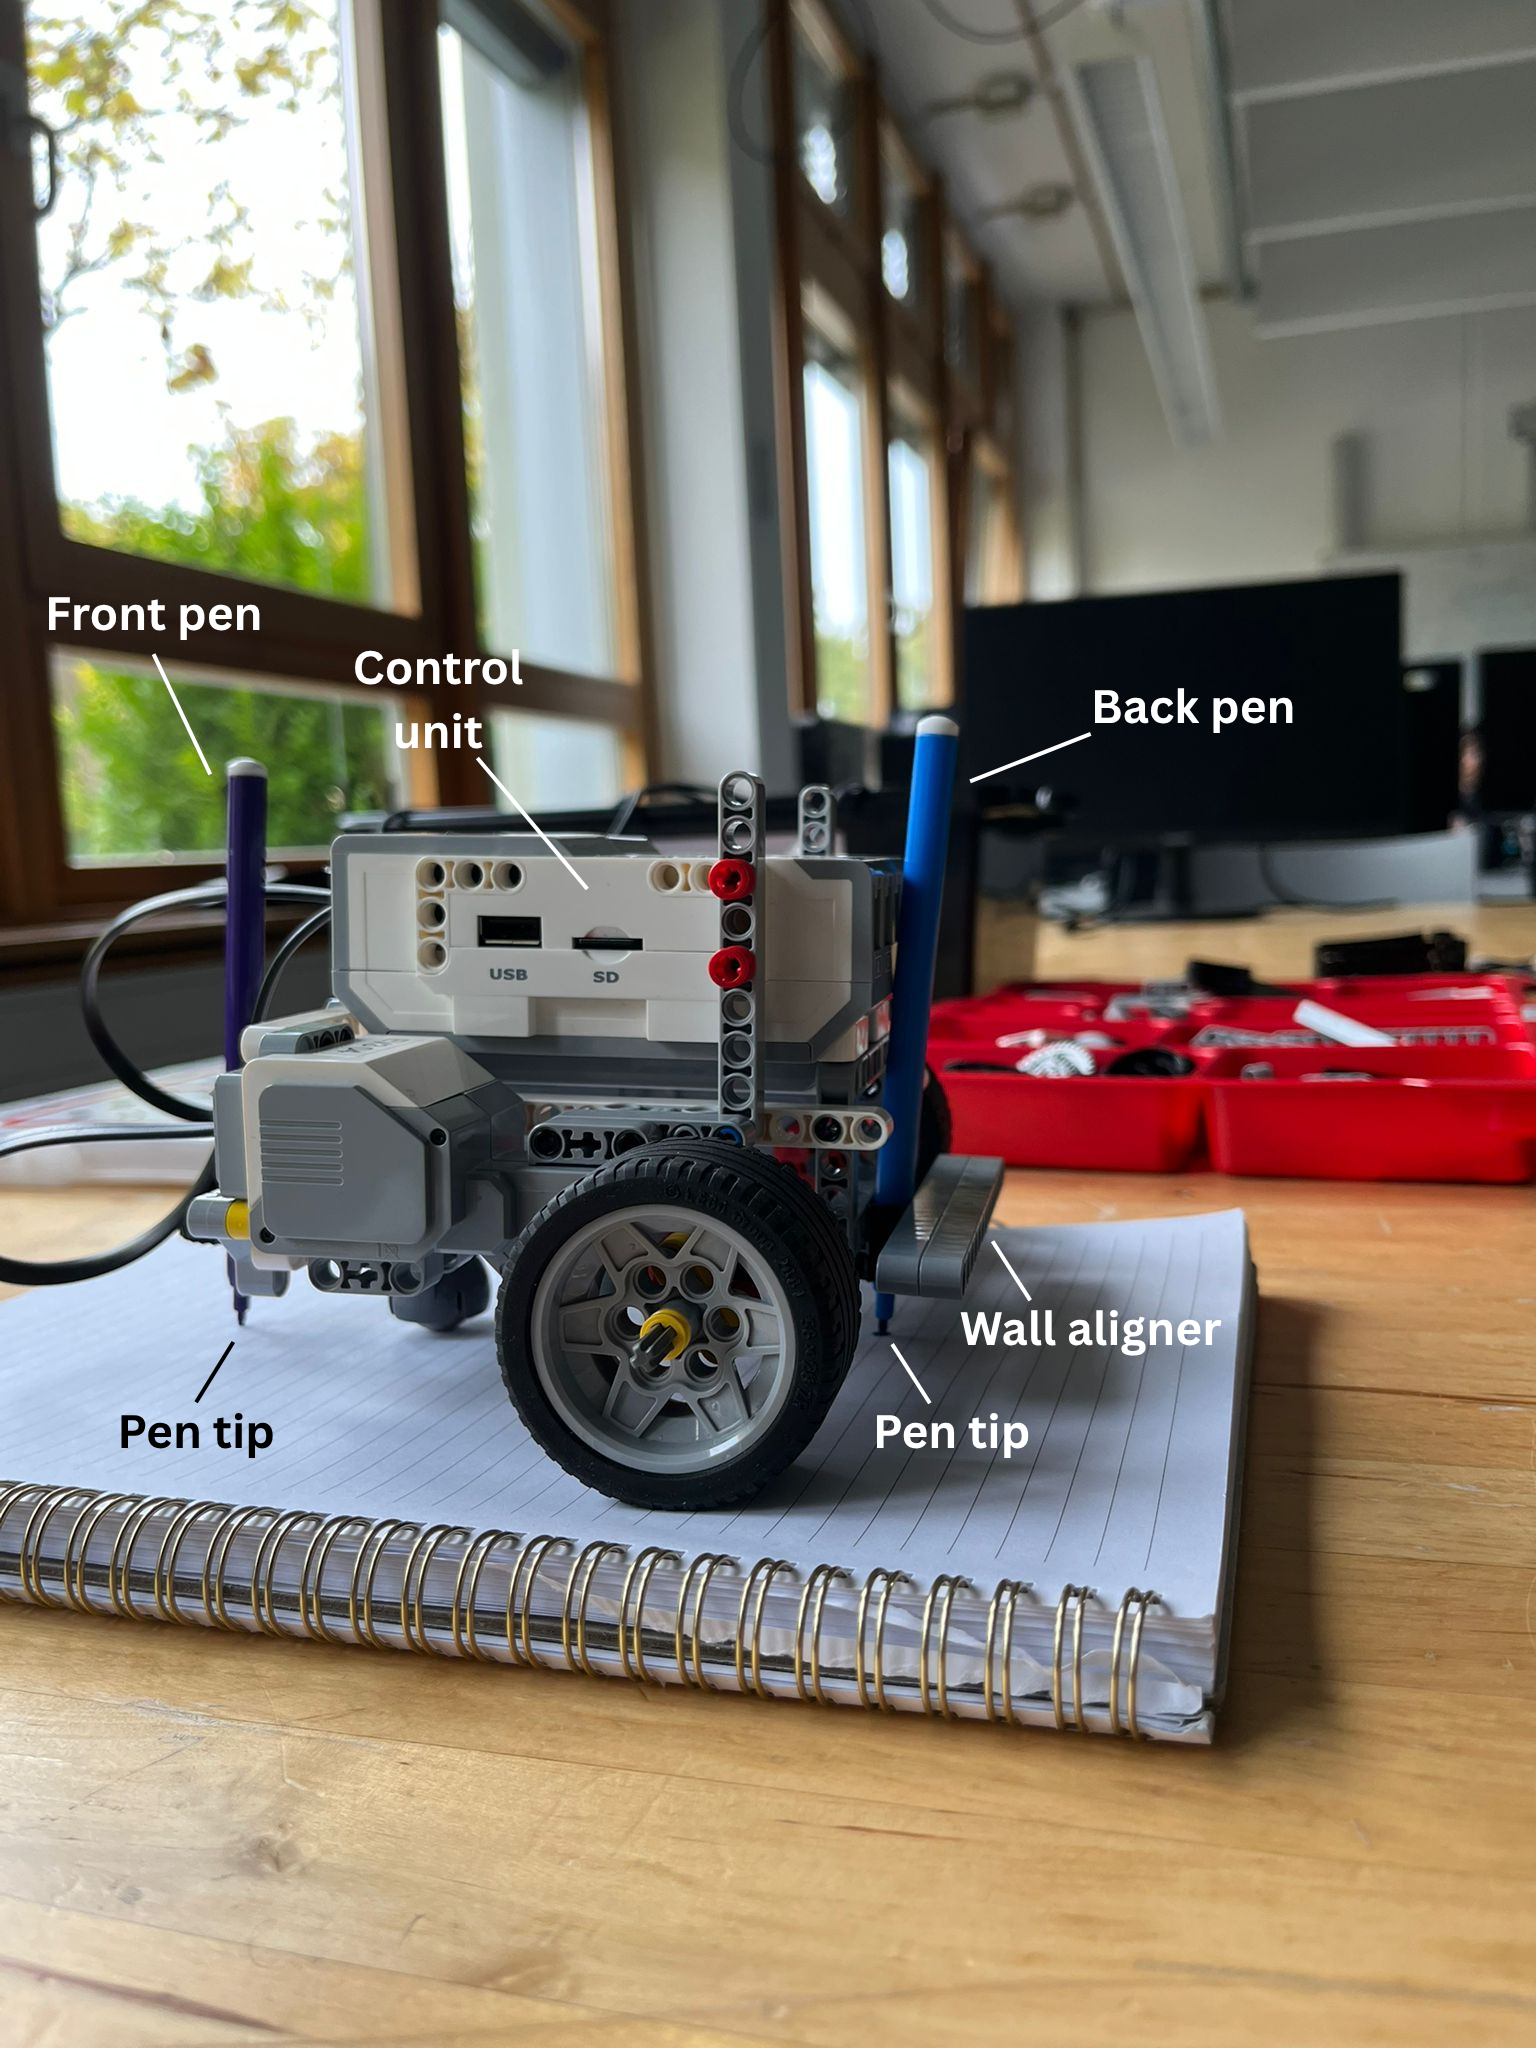
\includegraphics[width=0.8\linewidth]{figures/robot_angles/side.png}
        \caption{Side view of the robot}
        \label{fig:side_view}
    \end{figure}
    
    \begin{figure}[ht]
        \centering
        \includegraphics[width=0.8\linewidth]{figures/robot_angles/front.png}
        \caption{Front view of the robot}
        \label{fig:front_view}
    \end{figure}
    
    \begin{figure}[ht]
        \centering
        \includegraphics[width=0.8\linewidth]{figures/robot_angles/isometric.png}
        \caption{Isometric view of the robot}
        \label{fig:isometric_view}
    \end{figure}

    \begin{figure}[ht]
        \centering
        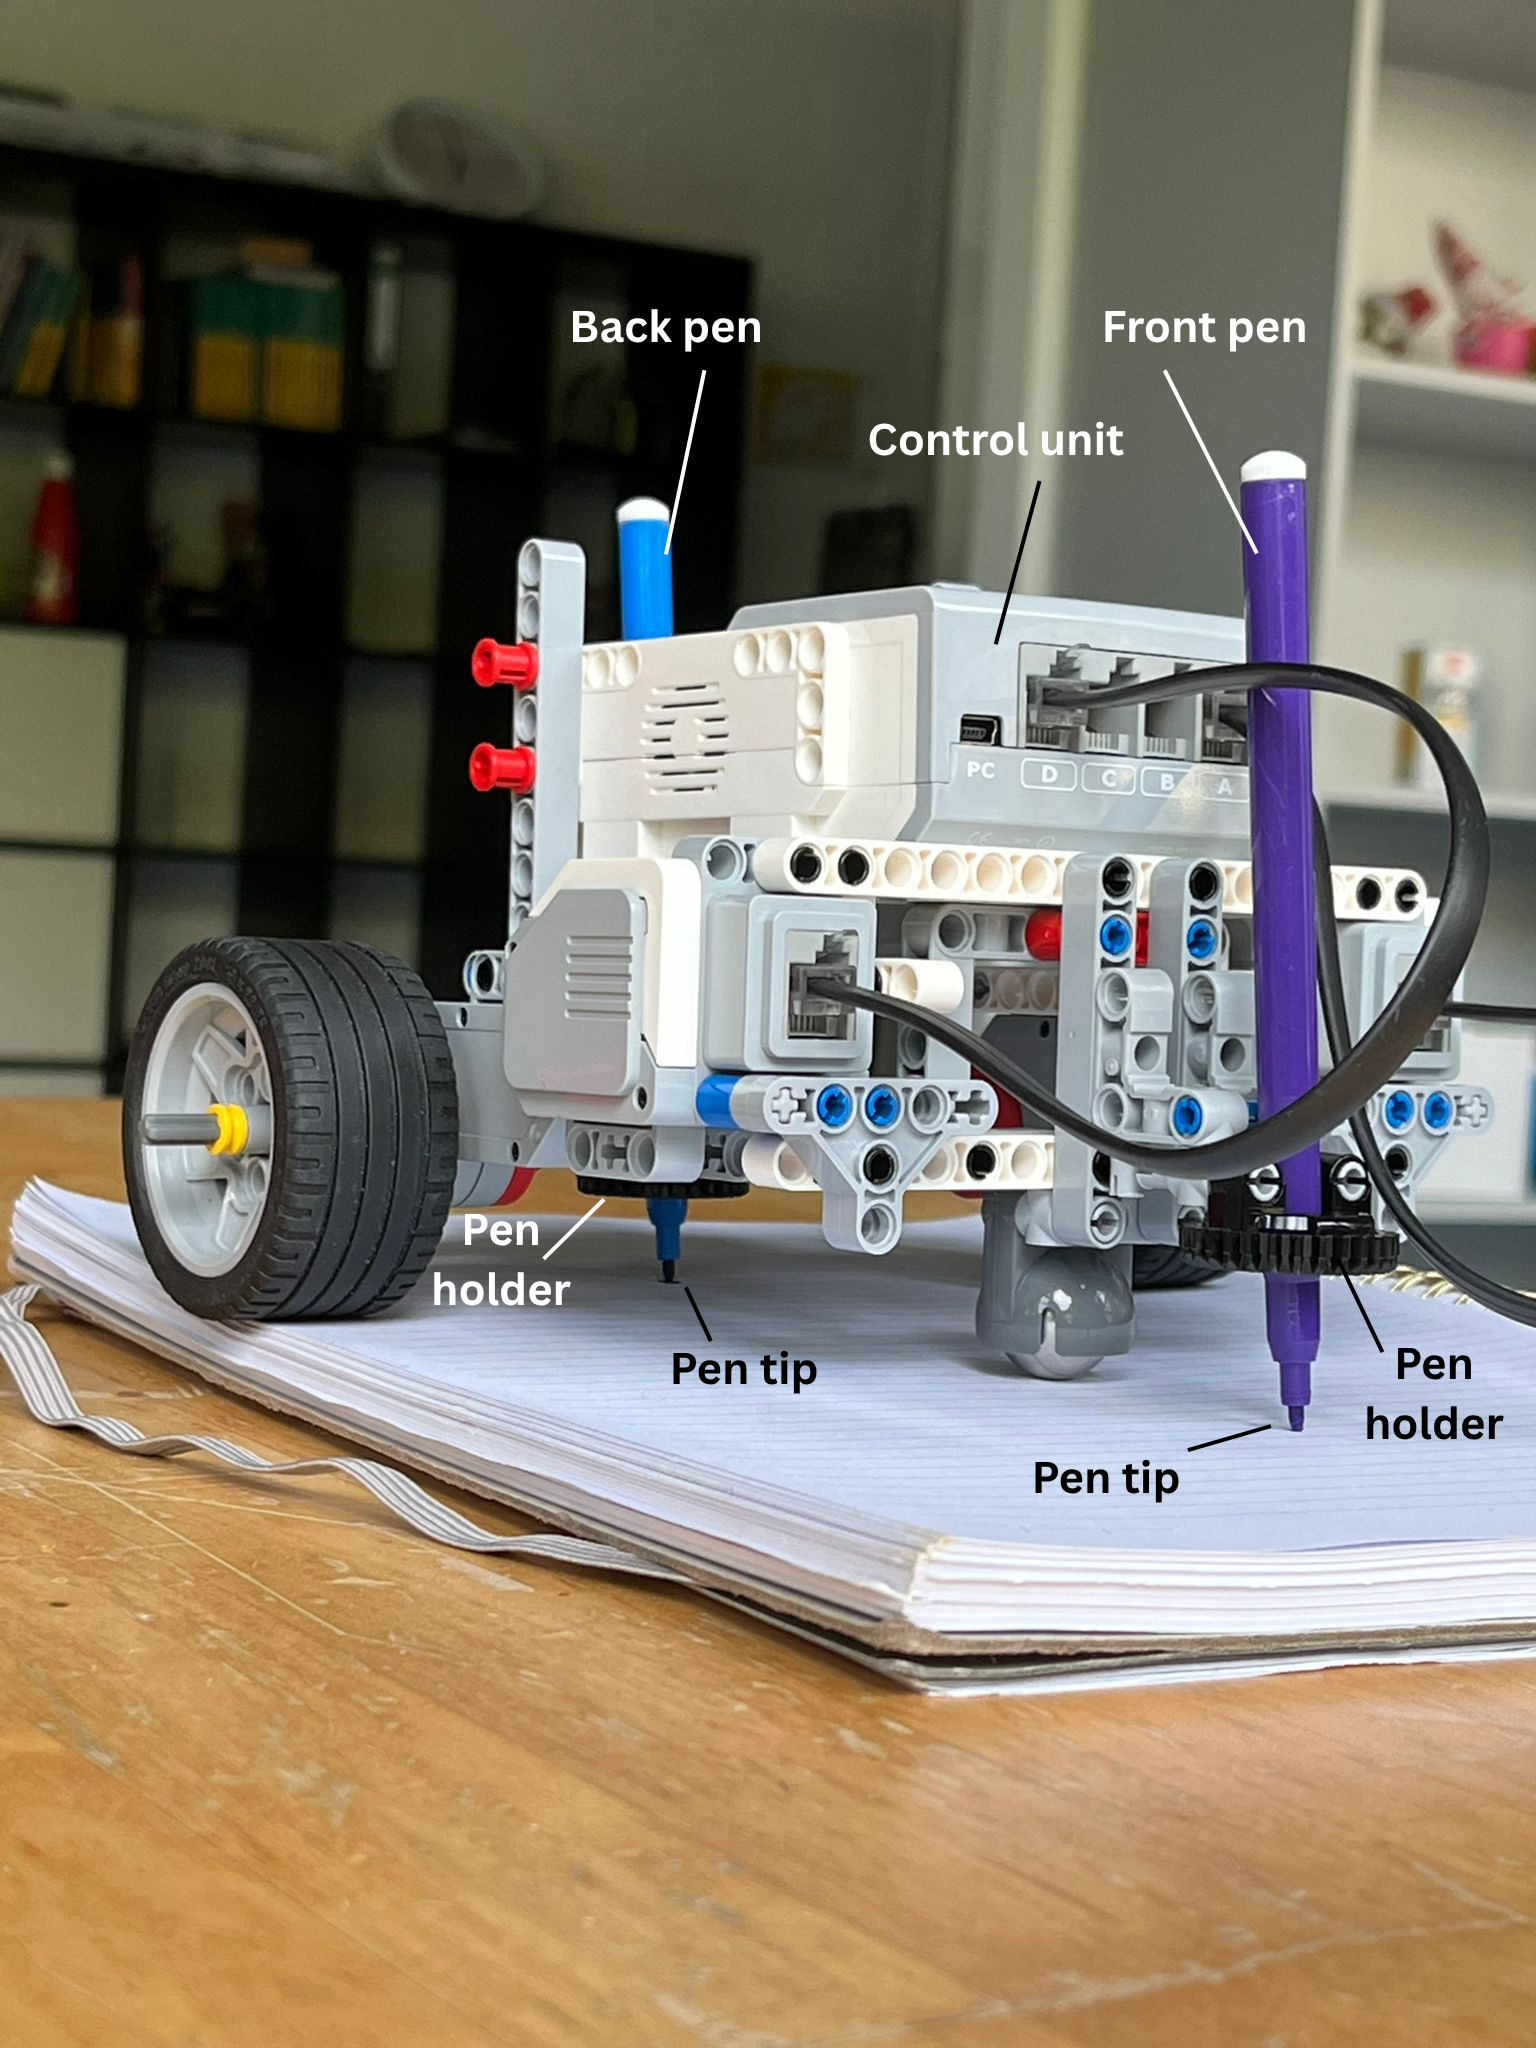
\includegraphics[width=0.8\linewidth]{figures/robot_angles/isometric2.png}
        \caption{Second isometric view of the robot}
        \label{fig:isometric2_view}
    \end{figure}   

    \begin{figure}[ht]
        \centering
        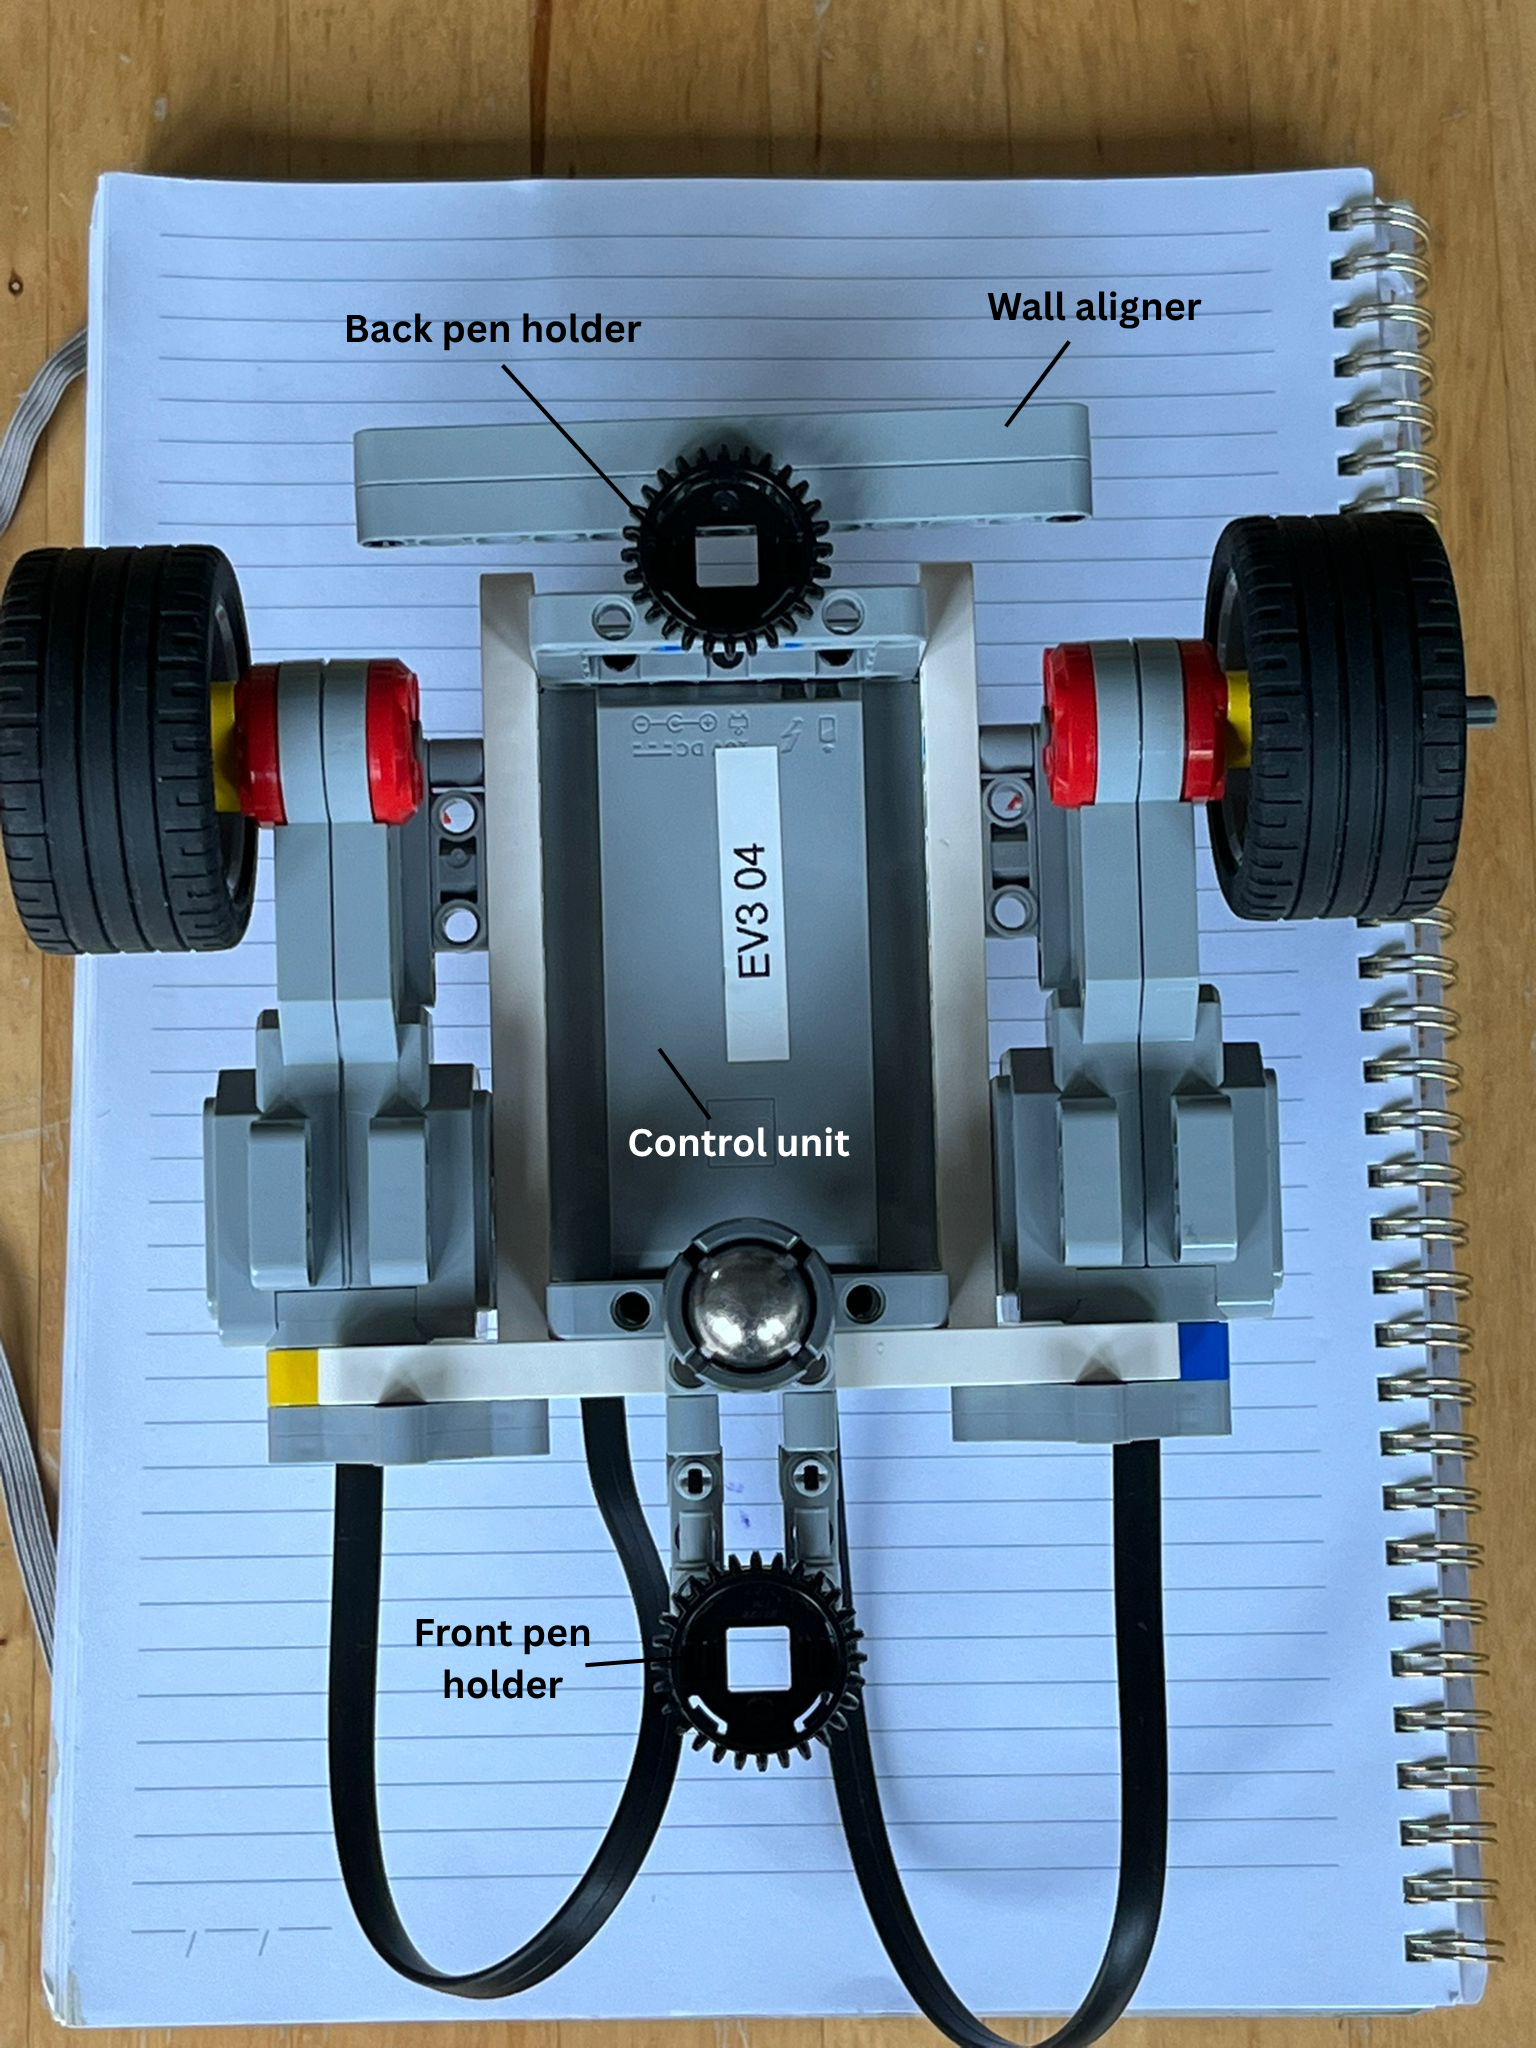
\includegraphics[width=0.8\linewidth]{figures/robot_angles/bottom.png}
        \caption{Bottom view of the robot}
        \label{fig:bottom_view}
    \end{figure} 

    \begin{figure}[ht]
        \centering
        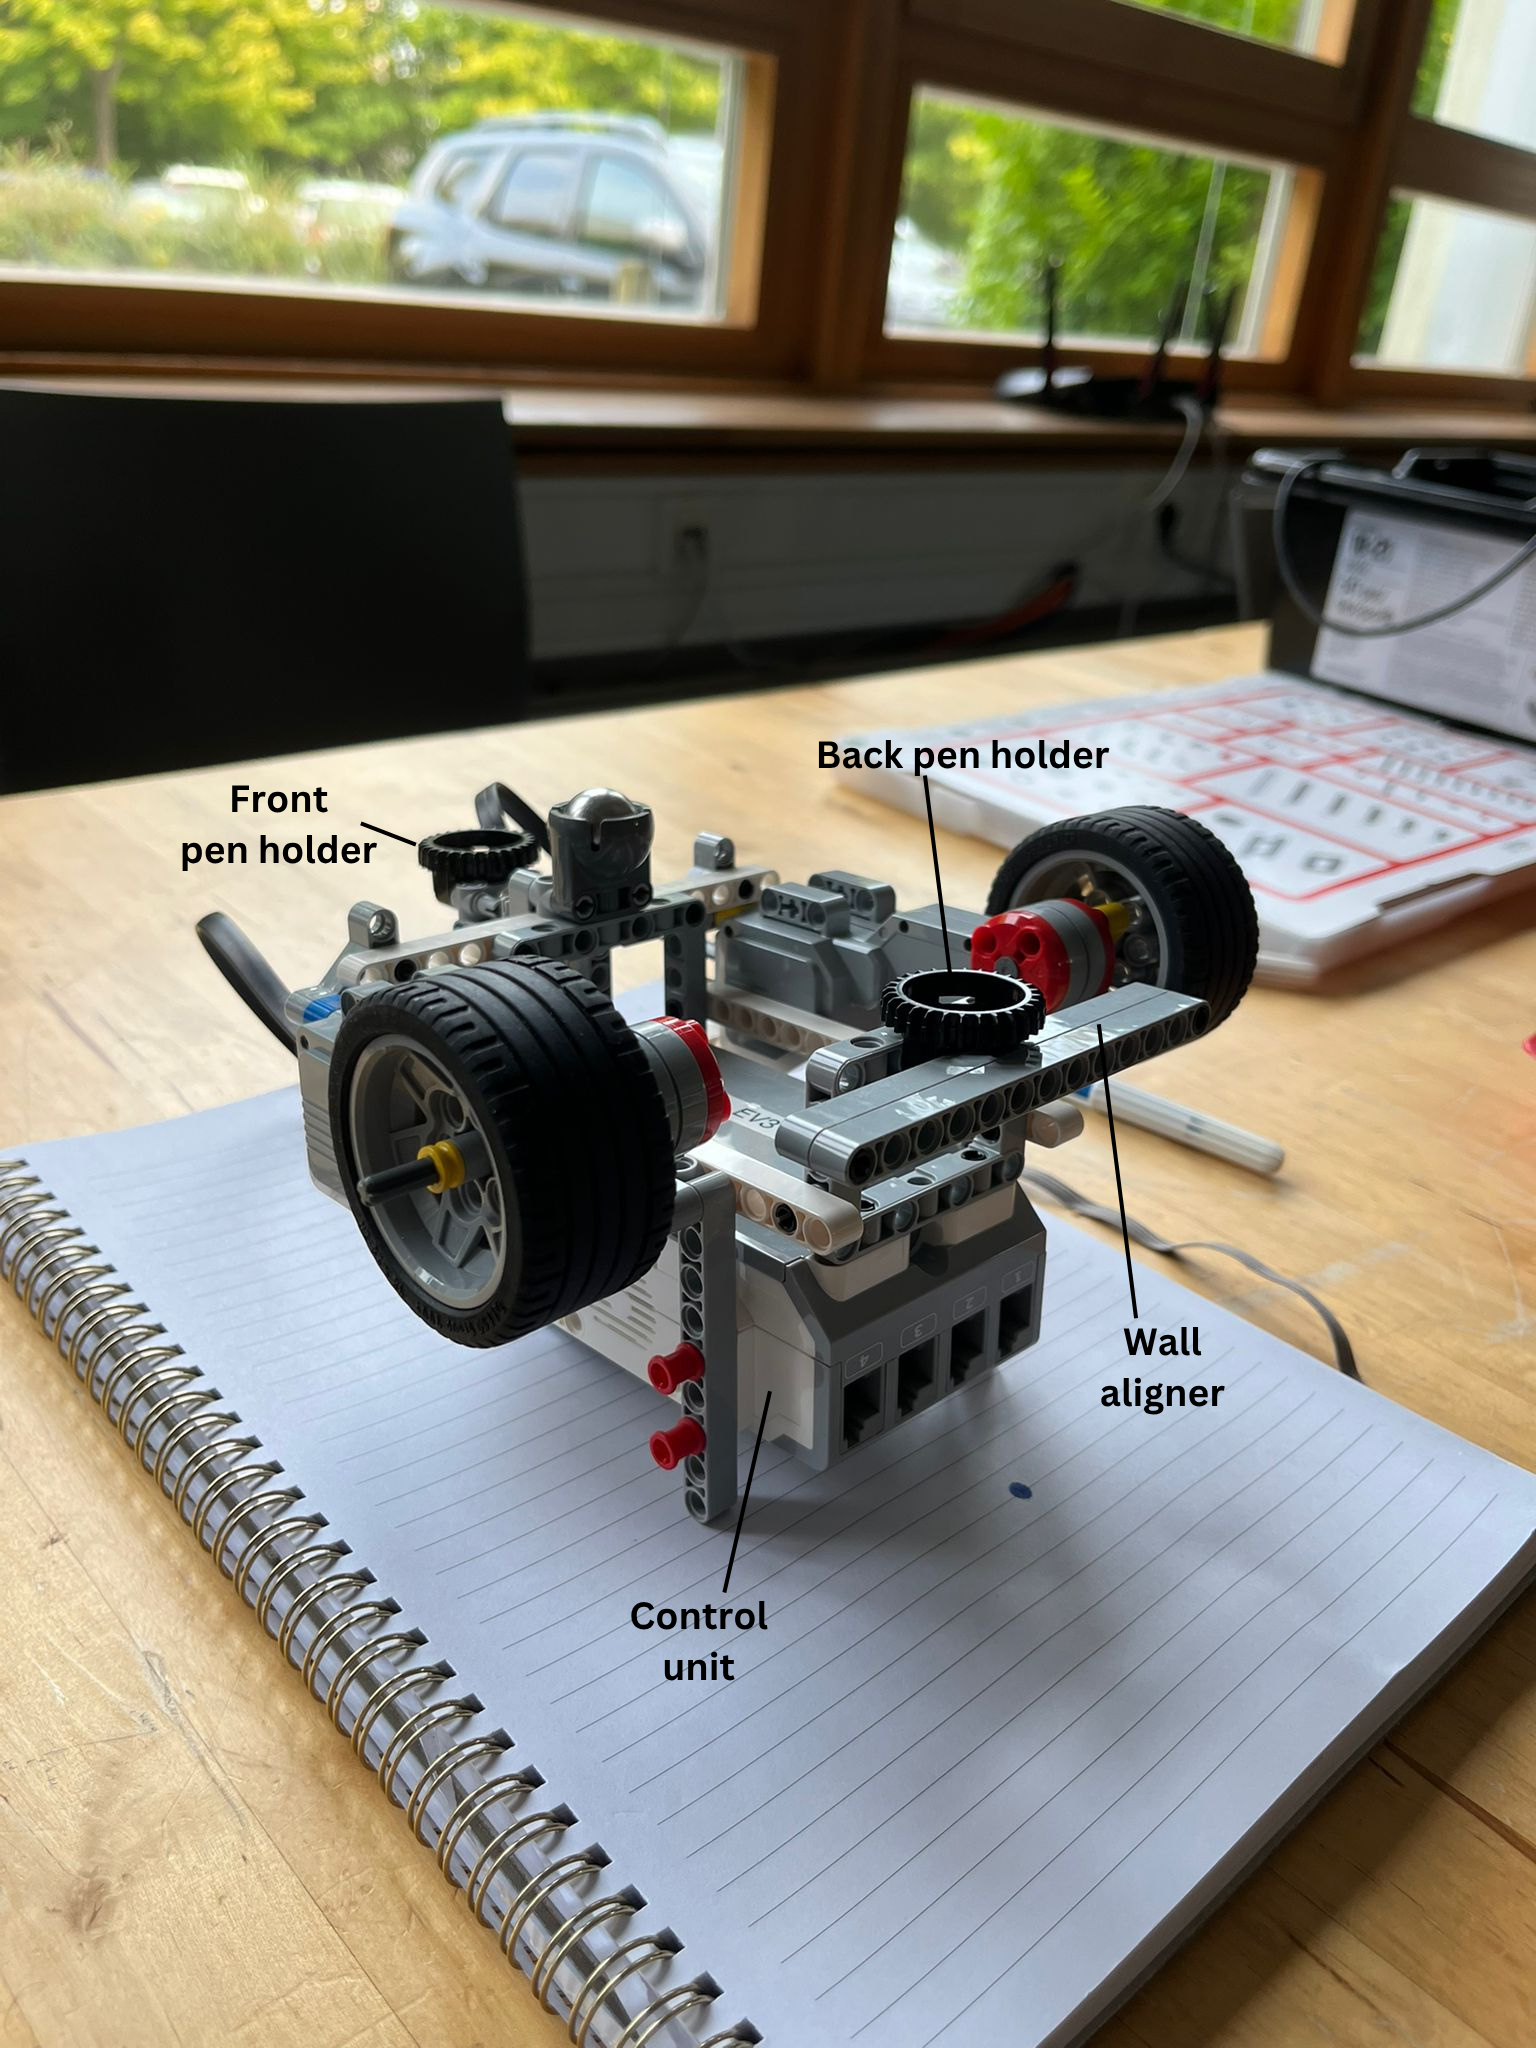
\includegraphics[width=0.8\linewidth]{figures/robot_angles/bottom_iso.png}
        \caption{Bottom-isometric view of the robot}
        \label{fig:bottom_iso_view}
    \end{figure} 


    The linear and angular velocities of a differential drive robot are given by:

    \begin{equation}
    v = \frac{r}{2} \left( \omega_r + \omega_l \right)
    \label{eq:linear_velocity}
    \end{equation}

    \begin{equation}
    \omega = \frac{r}{L} \left( \omega_r - \omega_l \right)
    \label{eq:angular_velocity}
    \end{equation}

    where $v$ is the linear velocity, $\omega$ the angular velocity, $r$ the wheel radius, 
    $L$ the distance between the wheels, and $\omega_r$, $\omega_l$ the angular velocities 
    of the right and left wheels, respectively.



    The figures in this section showcase various views of the robot that this team built. The construction and architecture of the robot is done in a way that the control unit comprises the middle part of the body. Since it is the most massive component of the robot, the control unit in the center, the center of gravity of the robot stays in approximately the middle of its body, which allows it to be stable. The two active wheels on both sides, along with the caster wheel, are placed while keeping the typical design of a differential drive robot in mind.
    The angles chosen for the views of the robot are such that each every detail of the robot's external body can be seen.
    In order to take measurements, the main components used were a pen holder, a pen, and a so-called 'wall aligner'. 
    When the robot would move, the front and back pens would have their tips touching and dragging along a surface such as a cardboard terrain.
    This would mark its trajectory using a combination of points and curved lines. Since the requirement of this assignment is
    to determine the pose of the robot, the two points formed from the pen tips making two blobs on the surface can allow for a straight line to be drawn connecting them. The centre point of the line, which can be calculated, can then serve as the position of the robot with its x and y axis. 
    The orientation with respect to the horizontal or x axis of the line can represent the desired orientation of the robot. 
    The pen holder is a circular piece we found in the lego kit with a hole in the middle that became suitable for its designated purpose.

    
    In order to ensure that the robot always starts from approximately the same pose in every trial of the experiment,
    the robot has a supposedly flat, long lego piece placed in a way such that its length is along a perpendicular axis to that of the rolling motion of the robot.
    The way this wall aligner works is by placing the robot in a corner of a room such that the wall aligner's flat surface completely pushes against the nearby wall surface in a way that there are no gaps between the wall aligner and the corresponding wall.


\cite{referenceexample}

\subsection{Estimates of the expected Precision}
PUT ERROR DUE TO MEASUREING HERE

\subsection{Jacobian Error Propagation}

Let $\mathbf{F}$ be a vector function, defining the \textbf{end pose} of the robot, calculated from two measured positions on a 2D plane, $\mathbf{x}_1$ and $\mathbf{x}_2$. The output components are defined such that $\mathbf{F}_1$ and $\mathbf{F}_2$ represent the position coordinates and $\mathbf{F}_3$ represents the angle of the end pose. It is important to note that $\mathbf{F}_3$ can only be used if $x_{1,2} \neq x_{2,2}$, otherwise the orientation is either $\frac{\pi}{2}$ for $x_{1,1} > x_{2,1}$, or $-\frac{\pi}{2}$ for $x_{1,1} < x_{2,1}$ The input vectors and the functional relationship are defined in Equations \ref{eq:x1x2} to \ref{eq:F}.

\begin{eqnarray}
	\mathbf{x}_1 &=& \begin{pmatrix} x_{1,1} \\ x_{1,2} \end{pmatrix} \label{eq:x1x2} \\
	\mathbf{x}_2 &=& \begin{pmatrix} x_{2,1} \\ x_{2,2} \end{pmatrix} \\
	\mathbf{F}(\mathbf{x}_1, \mathbf{x}_2) &=& \begin{pmatrix}
		\frac{1}{2}(x_{1,1} + x_{2,1}) \\
		\frac{1}{2}(x_{1,2} + x_{2,2}) \\
		\arctan\left(\frac{x_{2,1}-x_{1,1}}{x_{2,2}-x_{2,1}}\right)
	\end{pmatrix} \label{eq:F}
\end{eqnarray}

The propagation of uncertainty in the measured input coordinates requires the calculation of the \textbf{Jacobian matrix} $\mathbf{J}$. The total input vector $\mathbf{x} = (x_{1,1}, x_{1,2}, x_{2,1}, x_{2,2})^T$ is composed of all four scalar variables. Since $\mathbf{F}$ is a vector-valued function with three outputs and four inputs, the resulting Jacobian matrix $\mathbf{J}$ is a $3 \times 4$ matrix, presented in Equations \ref{eq:Jac} to \ref{eq:Jac_end}.

\begin{eqnarray}
	\mathbf{J} &=& \frac{\partial \mathbf{F}}{\partial \mathbf{x}} =
	\begin{pmatrix}
		\frac{\partial F_1}{\partial x_{1,1}} & \frac{\partial F_1}{\partial x_{1,2}} & \frac{\partial F_1}{\partial x_{2,1}} & \frac{\partial F_1}{\partial x_{2,2}} \\
		\frac{\partial F_2}{\partial x_{1,1}} & \frac{\partial F_2}{\partial x_{1,2}} & \frac{\partial F_2}{\partial x_{2,1}} & \frac{\partial F_2}{\partial x_{2,2}} \\
		\frac{\partial F_3}{\partial x_{1,1}} & \frac{\partial F_3}{\partial x_{1,2}} & \frac{\partial F_3}{\partial x_{2,1}} & \frac{\partial F_3}{\partial x_{2,2}}
	\end{pmatrix} \label{eq:Jac} \\
	&=& \begin{pmatrix}
		\frac{1}{2}               & 0                         & \frac{1}{2}               & 0                         \\
		0                         & \frac{1}{2}               & 0                         & \frac{1}{2}               \\
		\frac{x_{1,2}-x_{2,2}}{d} & \frac{x_{2,1}-x_{1,1}}{d} & \frac{x_{2,2}-x_{1,2}}{d} & \frac{x_{1,1}-x_{2,1}}{d}
	\end{pmatrix} \\
	d &=& (x_{1,1}-x_{2,1})^2+(x_{1,2}-x_{2,2})^2 \label{eq:Jac_end}
\end{eqnarray}

The \textbf{covariance matrix of the calculated end pose}, $\mathbf{C}_F$, is then determined from the input covariance matrix, $\mathbf{C}_x$, via the generalized error propagation formula, which can be seen in Equation \ref{eq:CF}.

\begin{equation}
	\mathbf{C}_F = \mathbf{J} \, \mathbf{C}_x \, \mathbf{J}^T \label{eq:CF}
\end{equation}
where $\mathbf{C}_x$ is the $4 \times 4$ covariance matrix of the input variables $(x_{1,1}, x_{1,2}, x_{2,1}, x_{2,2})$.




\end{document}
